\chapter{Materiais e Métodos}
\label{Materiais}

% Materiais e Métodos: descrição clara dos procedimentos e dos materiais adotados para o desenvolvimento do trabalho (sem resultados) incluindo sua adequação ao trabalho.
% Tem-se que responder às perguntas:
% 1) Está com um tamanho adequado (proporcional) à monografia?
% 2) Há informação suficiente e clara sobre os materiais e sobre os métodos adotados?
% Não há necessidade de reproduzir (copiar) as obras que embasam o trabalho e sim colocar o suficiente para o entendimento do trabalho e citar as referências.

Nesta seção serão apresentados os equipamentos necessários e métodos utilizados para o desenvolvimento do projeto. No caso dos equipamentos, serão apresentados todas as especificações técnicas e sua importância para o trabalho. Na seção destinada aos métodos, os algoritmos desenvolvidos para identificação e reconhecimento de objetos serão descritos.


%------------------------------------------------------------------------------------------------------------------------------------------------------------
\section{Materiais}

Com relação aos equipamentos é possível classificá-los em três grupos distintos: Câmeras estereoscópicas, Unidades de Processamento, e Equipamentos auxiliares.


%------------------------------------------------------------------------------------------------------------------------------------------------------------
\subsection{Câmeras estereoscópicas}

O projeto já utilizou duas câmeras estereoscópicas. Primeiramente, utilizou-se a \textit{webcam} Minoru(veja figura \ref{minoru}), visto que apresentava preço totalmente acessível e cumpria o requisito de realizar \textit{streaming} via USB. Deste modo, tornou-se um equipamento essencial para a implementação dos métodos para encontro de correspondências entre as câmeras. A tabela \ref{minoru_tab}	 apresenta as especificações da \textit{webcam}.

\begin{figure}[H]
	\centering
	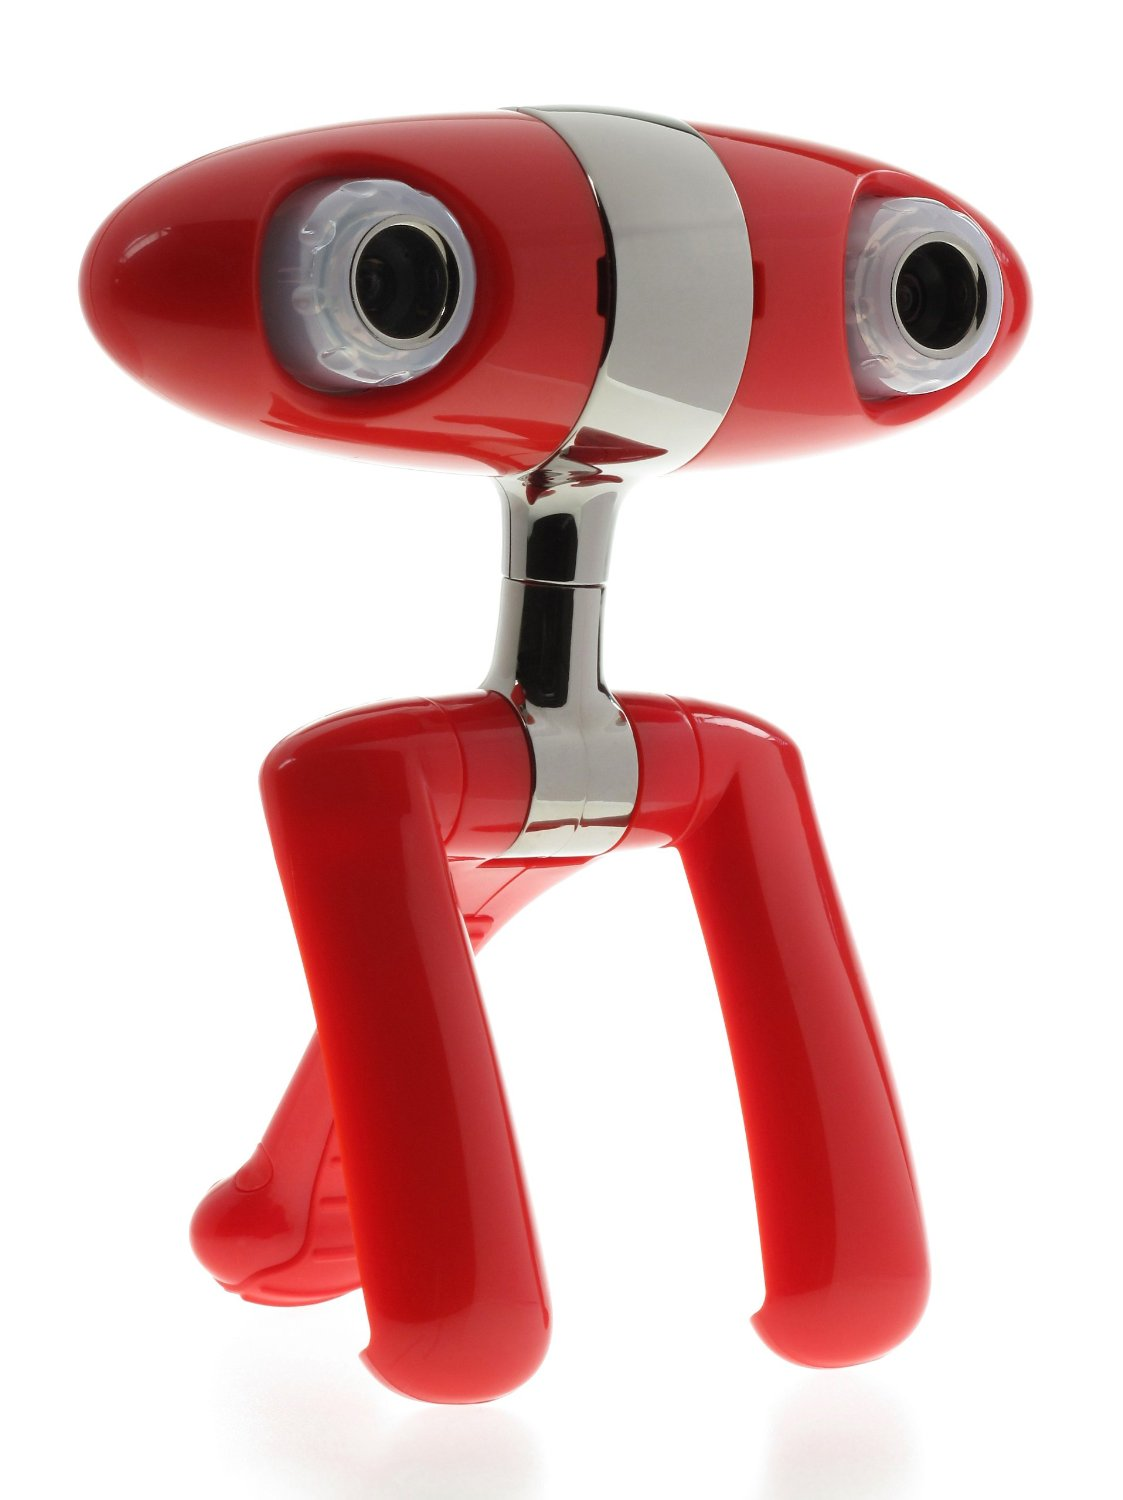
\includegraphics[scale=0.10]{./Resources/minoru.jpg}
	\caption{3D Webcam Minoru}
	\label{minoru}
\end{figure}

\begin{table}[]
\centering
\caption{Especificações - 3D Webcam Minoru}
\label{minoru_tab}
\begin{tabular}{ll}
\textbf{Sensor de Imagem}      & VGA CMOS Sensor  	\\
\textbf{Resolução Máxima}      & $800x600$        	\\
\textbf{Tamanho Linha de Base} & 6 cm             	\\
\textbf{Taxa de Captura}       & 30 fps             	\\
\textbf{Distância Focal}       & 10 cm até $\infty$	\\
\textbf{Campo de Visão}        & $42\degree$		   	\\
\textbf{Peso}				  & 249.48 g				\\
\end{tabular}
\end{table}

Atualmente, a câmera utilizada é uma câmera digital 3D W3 fabricada pela Fujifilm (veja figura \ref{fujiW3}). A primeira câmera foi substituída, pois o controlador USB não permitia que a webcam realizasse \textit{streaming} na máxima resolução. Deste modo, optou-se por uma câmera com maior resolução e que apresentasse lentes com baixa distorção. Entretanto, essa câmera não apresenta \textit{streaming} via USB, assim é necessário que os vídeos sejam processados \textit{offline}. Visto que o projeto preocupa-se principalmente na identificação de obstáculos, isso não oferece nenhuma desvantagem para o desenvolvimento do algoritmo. Todavia, para uma aplicação real, a câmera instalada no veículo deve apresentar esse aspecto. A tabela \ref{fujiW3_tab} apresenta as especificações da câmera.

\begin{table}[]
\centering
\caption{Especificações - Câmera Digital Fujifilm FinePix Real 3D W3}
\label{fujiW3_tab}
\begin{tabular}{ll}
\textbf{Sensor de Imagem}      & 10 MP CCD Sensor  	\\
\textbf{Resolução Máxima}      & $1280x720$        	\\
\textbf{Tamanho Linha de Base} & 7.5 cm             	\\
\textbf{Taxa de Captura}      & 24 - 30 fps          \\
\textbf{Distância Focal}       & 60 cm até $\infty$	\\
\textbf{Peso}       		      & 250g					\\
\end{tabular}
\end{table}

\begin{figure}[H]
	\centering
	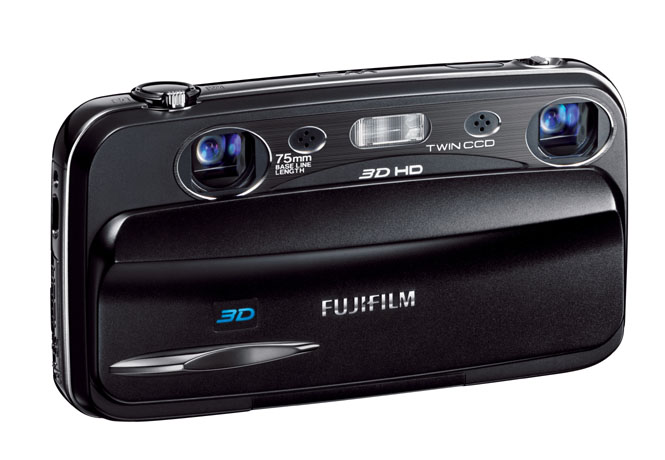
\includegraphics[scale=0.35]{./Resources/fujiW3.jpg}
	\caption{Câmera Digital Fujifilm FinePix Real 3D W3}
	\label{fujiW3}
\end{figure}


%------------------------------------------------------------------------------------------------------------------------------------------------------------
\subsection{Unidades de Processamento}

Visto que este trabalho também busca a implementação dos algoritmos de detecção de obstáculos em quadricópteros, tem-se como objetivo sua implementação para Linux embarcado (\textit{Embedded Linux}).Abaixo estão apresentadas as plataformas que serão utilizadas para este propósito.


%------------------------------------------------------------------------------------------------------------------------------------------------------------
\subsubsection{BBB}

A primeira a ser utilizada e estudada é a plataforma aberta BeagleBone Black, ilustrada pela figura \ref{bbb}. Esta plataforma foi escolhida devido ao seu tamanho reduzido, podendo ser facilmente embarcada, isto é, é possível adaptá-la mecanicamente ao veículo, e ao seu poder de processamento, utiliza Cortex-A8 operando à 1 GHz. A tabela \ref{bbb_tab} apresenta as especificações da plataforma.

\begin{table}[]
\centering
\caption{Especificações - BeagleBone Black}
\label{bbb_tab}
\begin{tabular}{ll}
\textbf{Processador}           & 1GHz TI Sitara AM3359 ARM Cortex-A8			\\
\textbf{RAM}                   & 512 MB DDR3L @ 400 MHz					\\
\textbf{Armanezamento}         & 2 GB on-board eMMC, MicroSD				\\
\textbf{Sistemas Operacionais} & Angstrom (Default), Ubuntu, Android, dentre outros...	\\
\textbf{Consumo de energia}    & 210-460 mA @ 5V					\\
\textbf{Pinos de GPIO}         & 65/92 pinos						\\
\textbf{Periféricos}           & 1 USB Host, 1 Mini-USB Client, 1 10/100 Mbps Ethernet                                 
\end{tabular}
\end{table}

\begin{figure}[H]
	\centering
	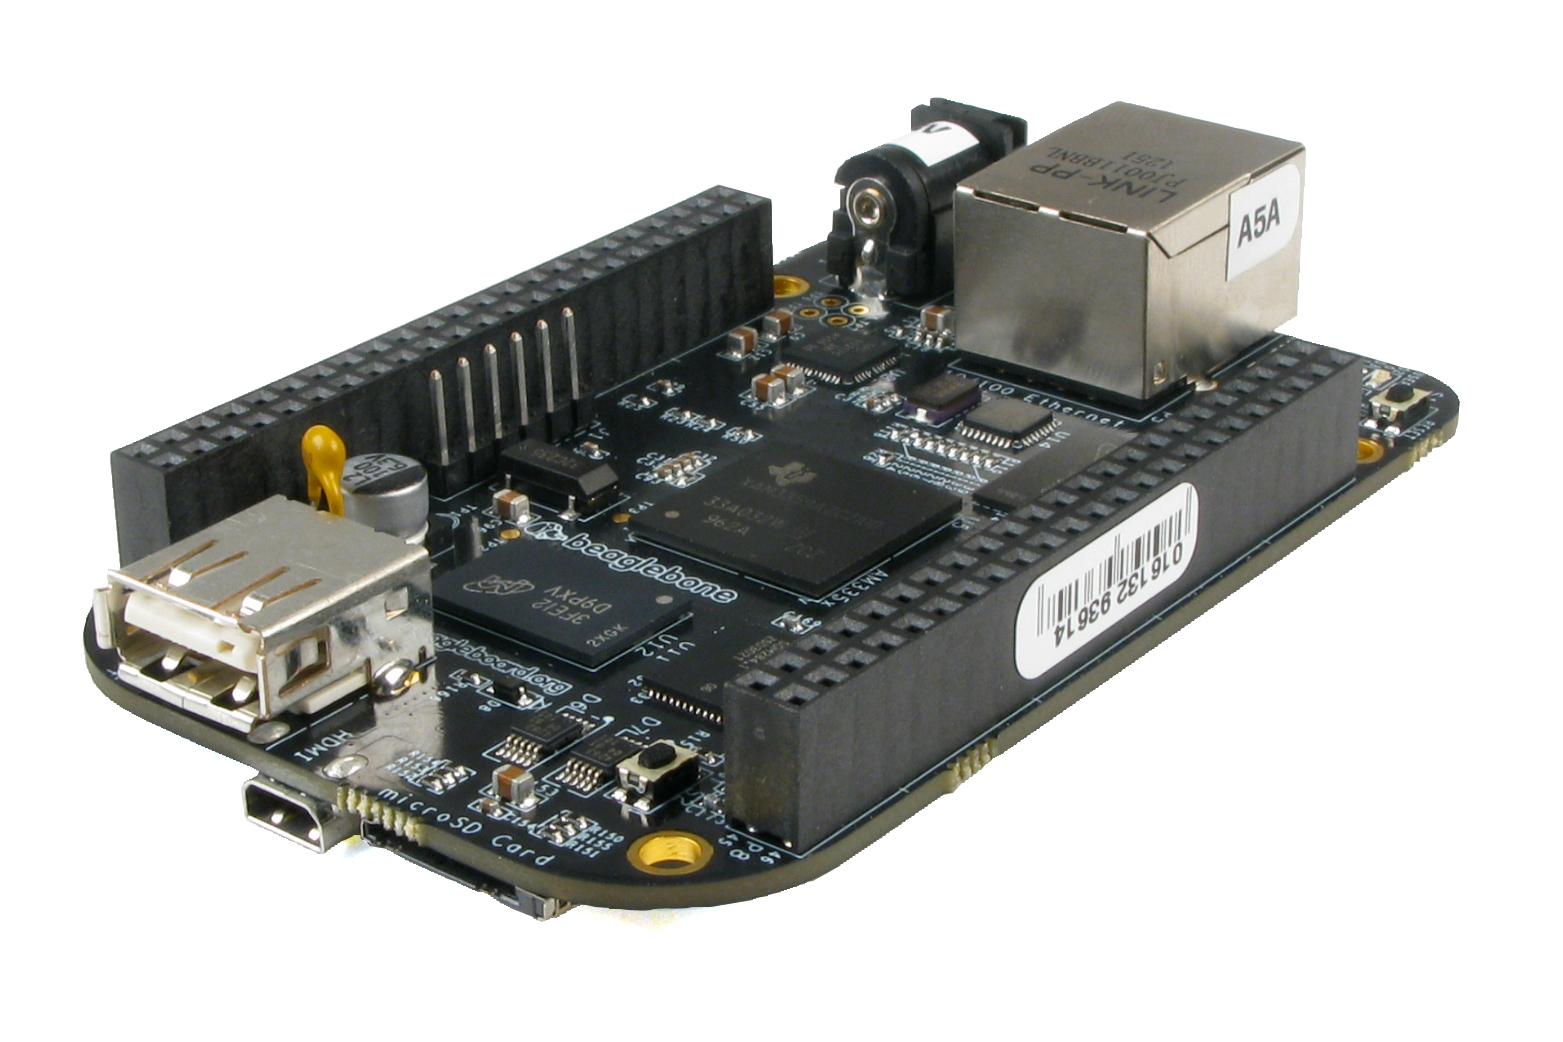
\includegraphics[scale=0.10]{./Resources/bbb.jpg}
	\caption{Plataforma de Desenvolvimento - BeagleBone Black}
	\label{bbb}
\end{figure}


%------------------------------------------------------------------------------------------------------------------------------------------------------------
\subsubsection{Jetson TK1}

A segunda a ser utilizada e estudada é a plataforma Jetson TK1 produzida pela NVIDIA, figura \ref{jetson_tk1}. Essa plataforma conta com um processador de 32-bits Tegra K1 baseado na tecnologia ARM Cortex-A15. O motivo pelo qual esta plataforma foi escolhida é devido ao seu poder de processamento gráfico, visto que apresenta 192 núcleos gráficos, sendo assim adequada para aplicações envolvendo processamento de imagens. A tabela \ref{jetson_tk1_tab} apresenta as especificações da plataforma. Outro fator interessante desta plataforma é que ela oferece suporte à tecnologia CUDA, a qual será discutida mais adiante.

\begin{table}[]
\centering
\caption{Especificações - Jetson TK1}
\label{jetson_tk1_tab}
\begin{tabular}{ll}
\textbf{Processador}           & NVIDIA 2.32GHz ARM quad-core Cortex-A15              \\
\textbf{Processador Gráfico}   & NVIDIA Kepler "GK20a" GPU  with 192 SM3.2 CUDA cores \\
\textbf{DRAM}                  & 2GB DDR3L 933MHz EMC x16 using 64-bit data width     \\
\textbf{Armanezamento}         & 16GB fast eMMC 4.51 (routed to SDMMC4)               \\
\textbf{Sistemas Operacionais} & Platforma 64-bit Linux Ubuntu 14.04                  \\
\textbf{Consumo de energia}    & 0.6W to 3W @ 12 V                                    \\
\textbf{Pinos de GPIO}         & 7 x GPIO pins (1.8V)                                 \\
\textbf{Periféricos}           & USB, mini-PCIe, SATA, SD-card, HDMI, audio          
\end{tabular}
\end{table}

\begin{figure}[H]
	\centering
	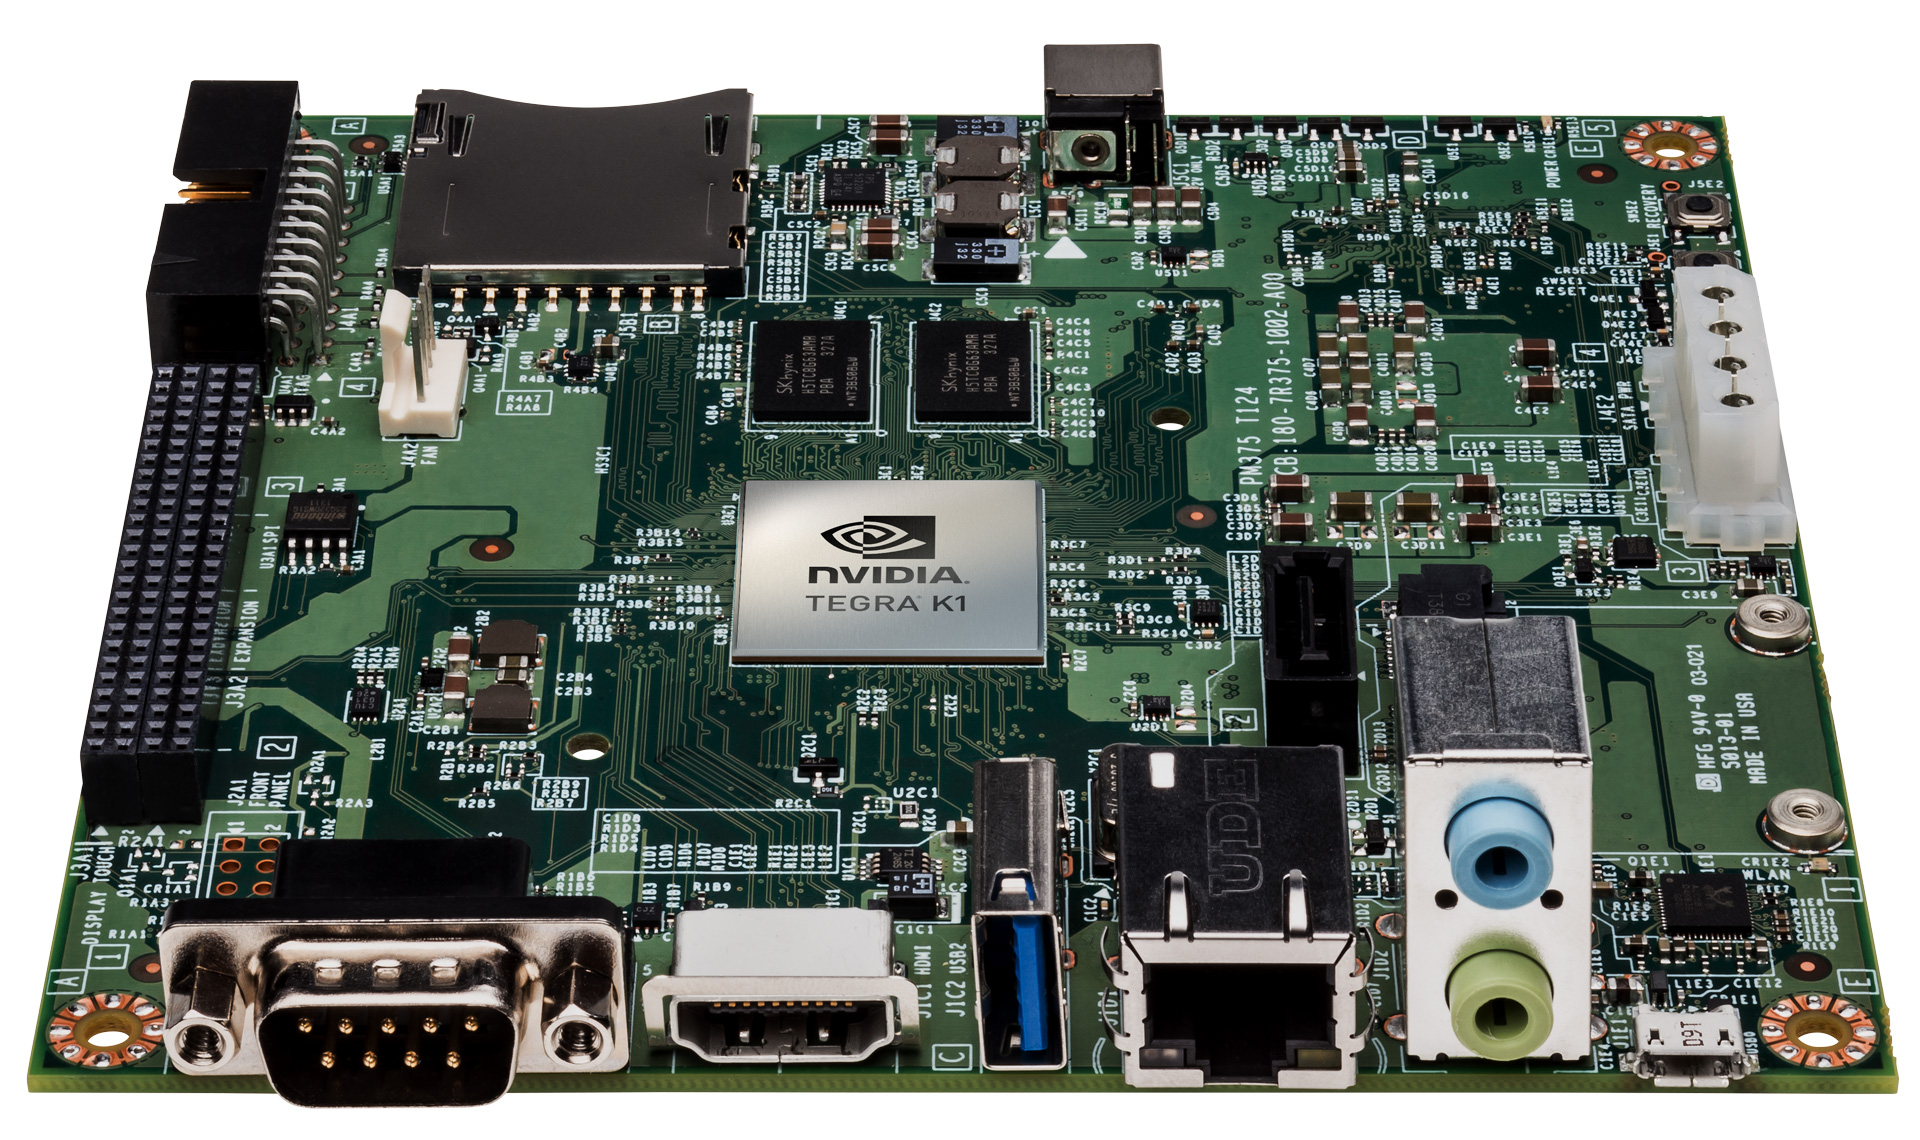
\includegraphics[scale=0.10]{./Resources/jetson_tk1.jpg}
	\caption{Plataforma de Desenvolvimento - Jetson TK1}
	\label{jetson_tk1}
\end{figure}


%-----------------------------------------------------------------------------------------------------------------------------------------------------------------------------------------------
\subsection{Equipamentos auxiliares}

Abaixo estão apresentados os equipamentos auxiliares para o desenvolvimento do trabalho. 

Os métodos para a identificação de correspondências entre as câmeras requerem que a imagem estejam calibradas e retificadas. Por conta disso, utiliza-se o padrão de calibração de dimensão 7x10, apresentado na figura \ref{calibration_pattern}, para este propósito. Deste modo, é possível caracterizar as distorções das lentes, parâmetros intrínsecos, e o posicionamento de uma das câmeras com relação a outra, parâmetros extrínsecos.  

\begin{figure}[H]
	\centering
	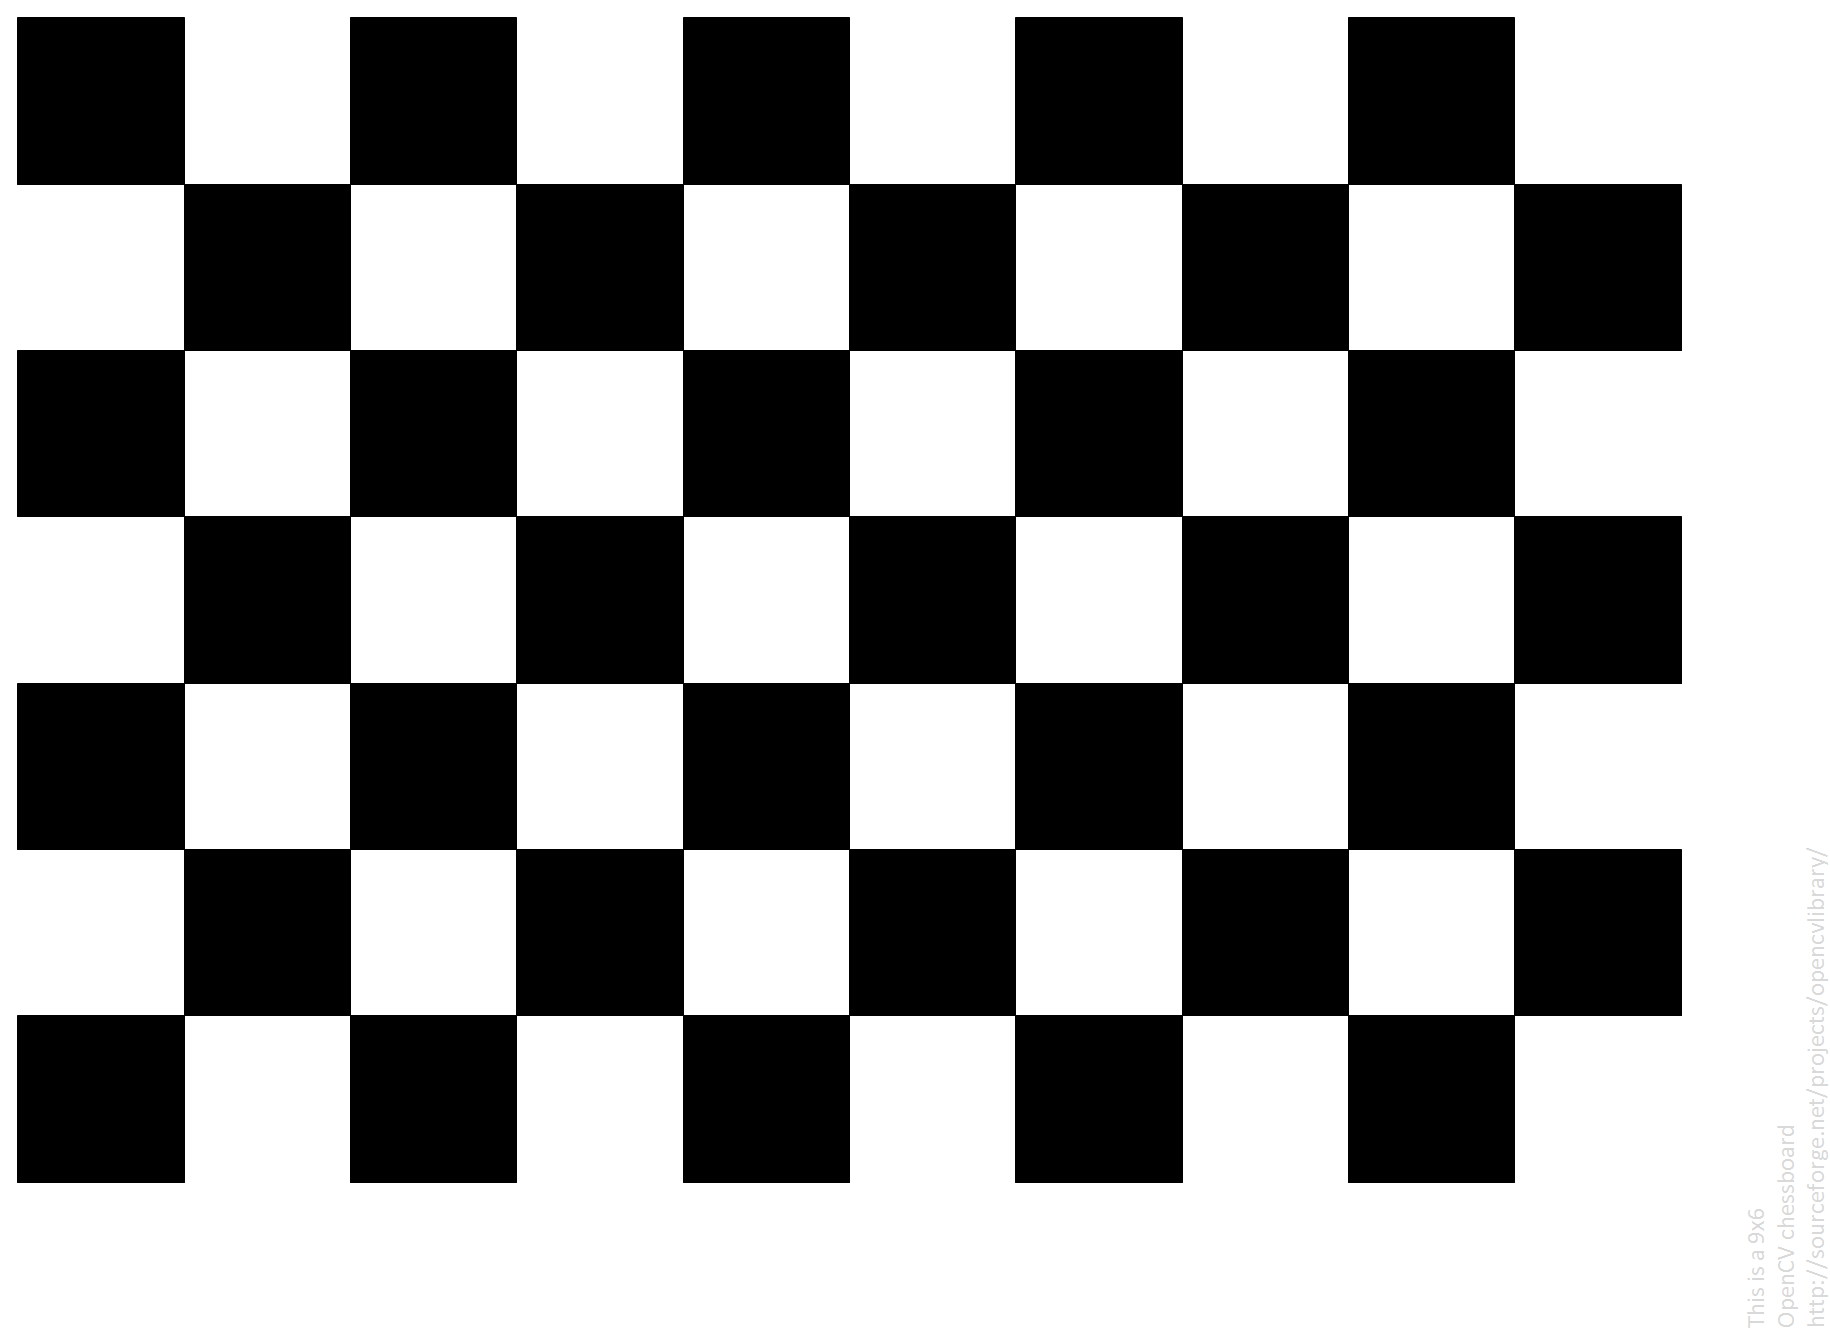
\includegraphics[scale=0.10]{./Resources/calibration_pattern.png}
	\caption{Padrão de Calibração}
	\label{calibration_pattern}
\end{figure}

A motivação deste trabalho é a sua utilização em veículos aéreos. Por conta disso, é indispensável que se tenha algum desses veículos. O trabalho conta com a utilização de um quadricóptero produzido pela 3DR, porém este apresenta modificações visando o seu desenvolvimento para navegação autônoma. Deste modo, tem-se a adição de \textit{propellers guards}, objetivando o aumento da segurança do veículo e das pessoas que o operam. Além disso, o \textit{drone} conta com suportes para a câmera estereoscópica e para a plataforma embarcada. Como pode ser observado pela figura \ref{quad_camera_support}, todas as peças foram produzidas utilizando impressora 3D.

\begin{figure}[H]
	\centering
	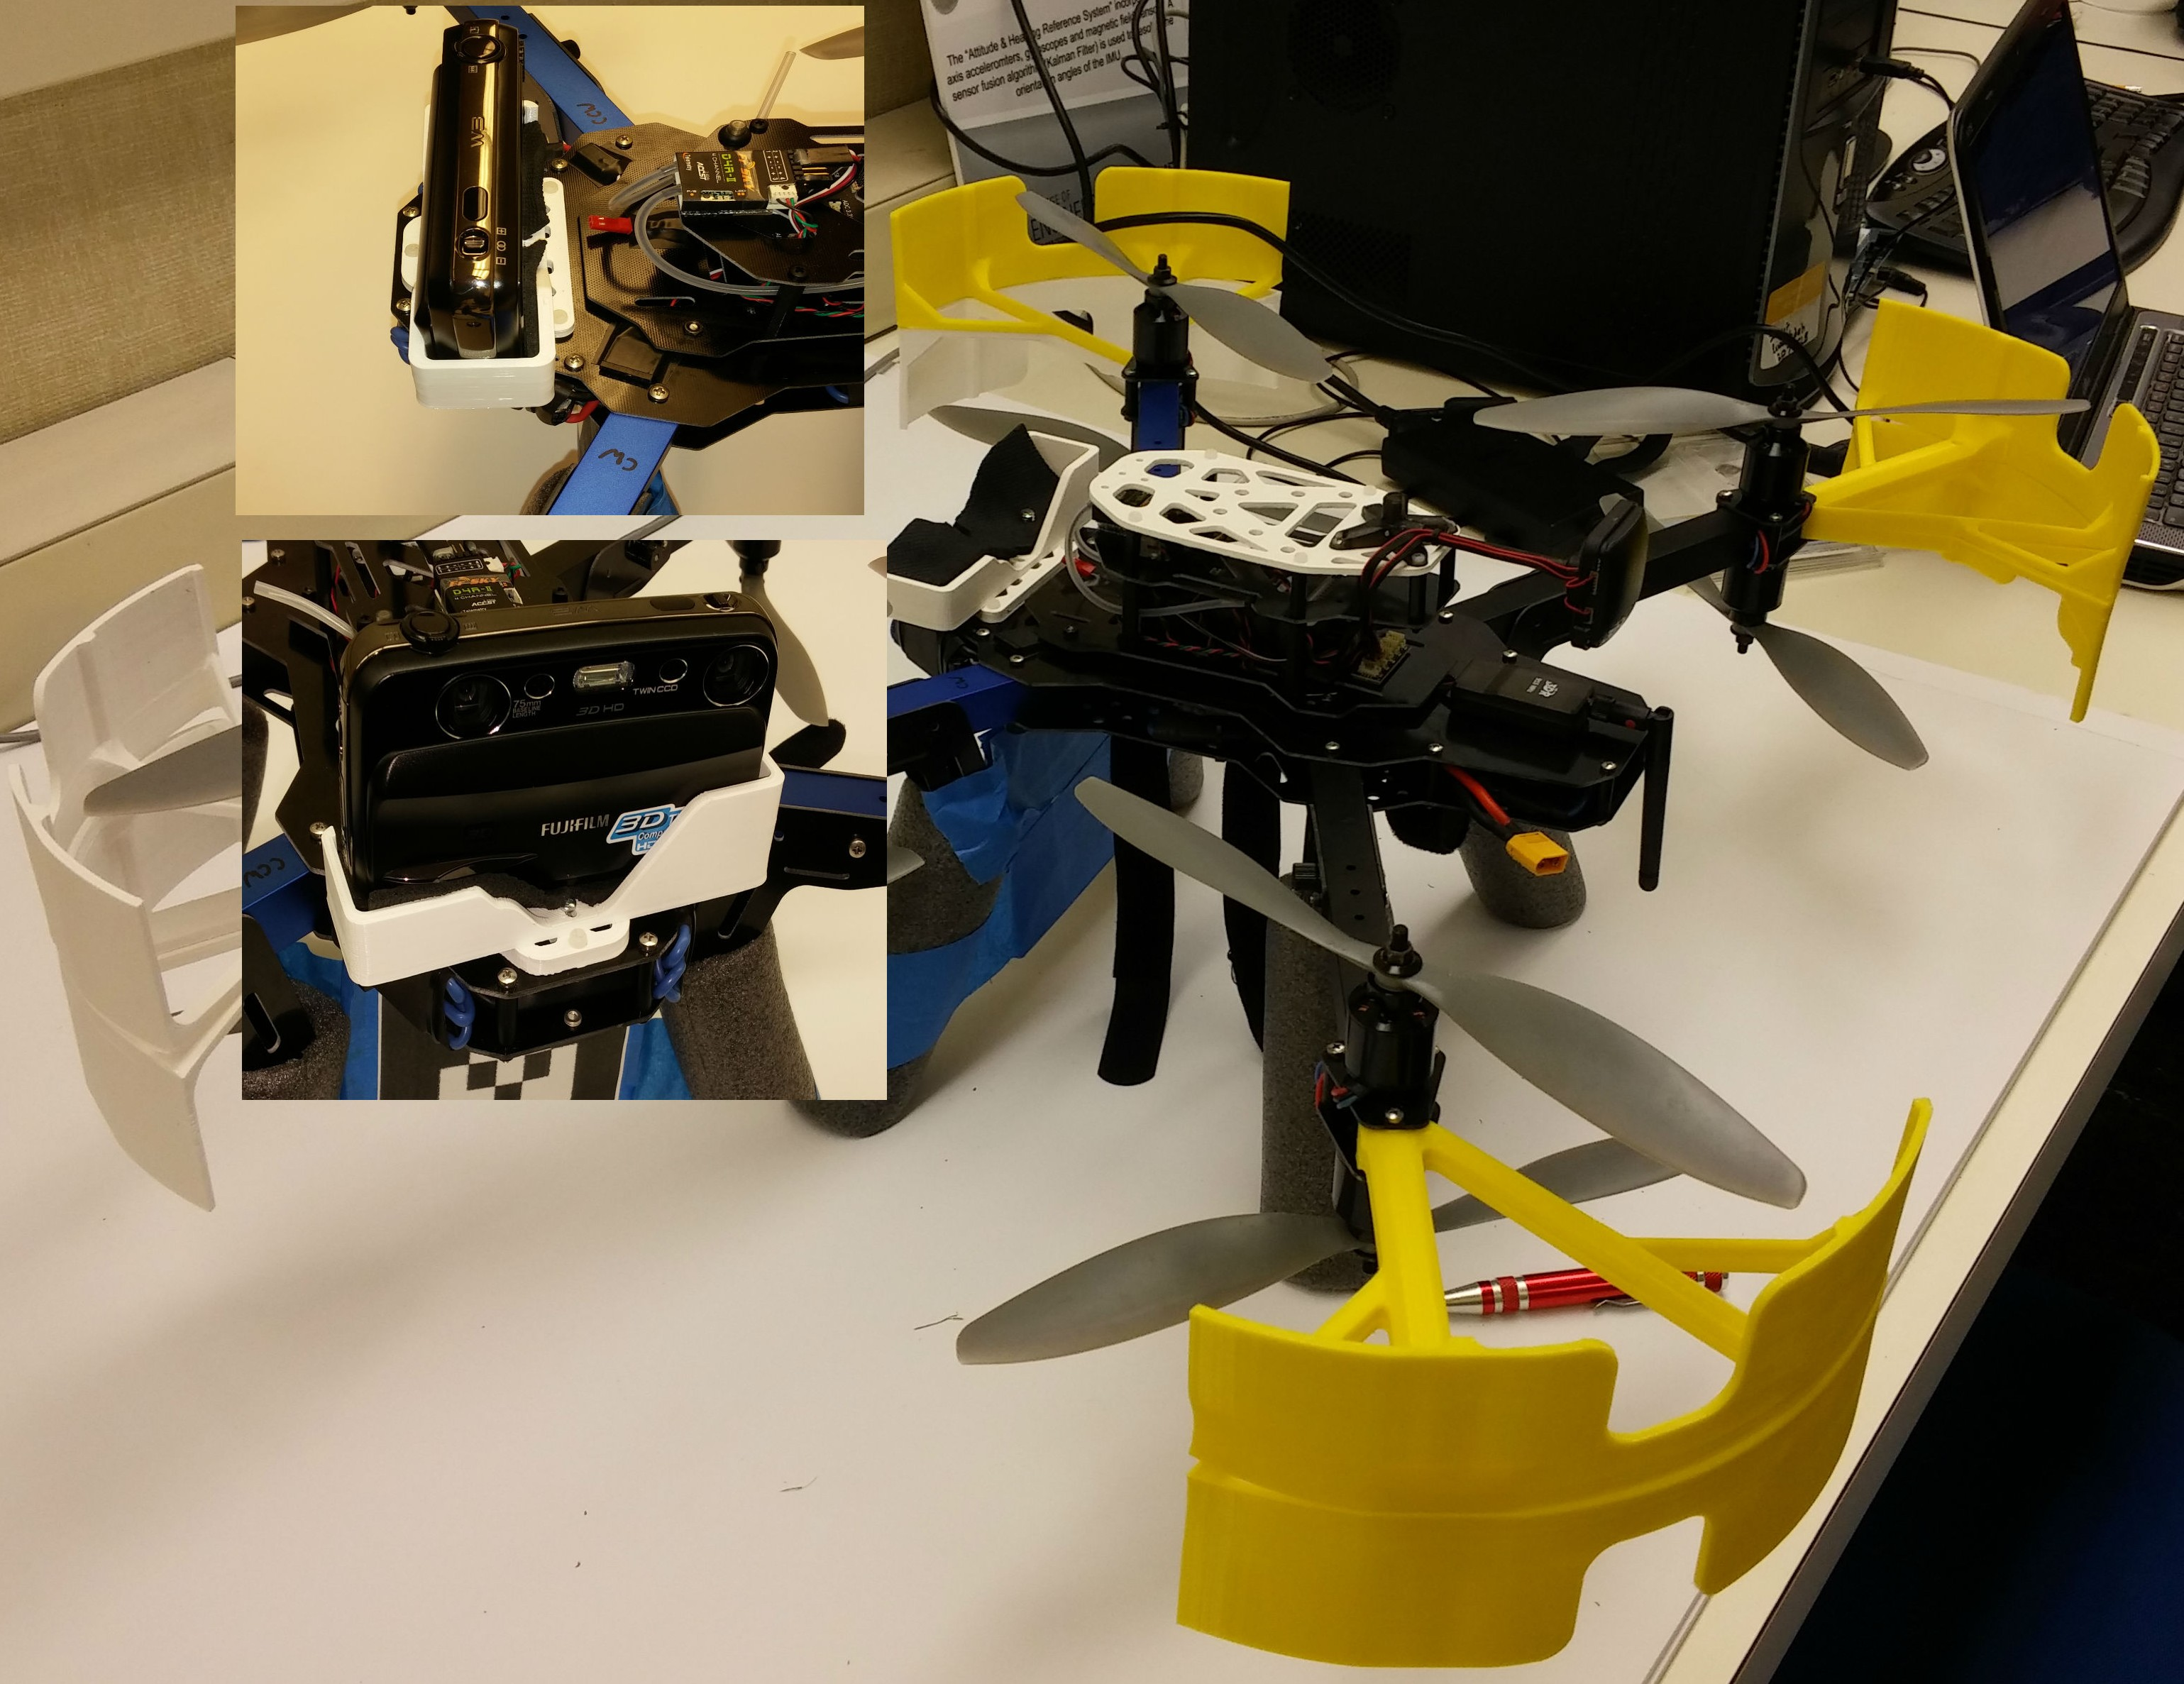
\includegraphics[scale=0.10]{./Resources/quad_camera_support.jpg}
	\caption{Quadricóptero 3DR X8 com suporte para a Câmera 3D}
	\label{quad_camera_support}
\end{figure}


%-----------------------------------------------------------------------------------------------------------------------------------------------------------------------------------------------
\section{Métodos}

Nesta seção serão apresentados os cenários e os métodos utilizado para o desenvolvimento do algoritmo para a detecção de obstáculos.

%-----------------------------------------------------------------------------------------------------------------------------------------------------------------------------------------------
\subsection{Cenários}

O algoritmo de detecção de obstáculos desenvolvido tenta contornar todas as adversidades propostas pelos seguintes cenários. Propôs-se que ele deve ser flexível à variações na luminosidade, capaz de detectar obstáculos estáticos e móveis, e ser imune à vibrações. Deste modo, dois cenários em ambiente confinado e um em ambiente aberto foram analisados. Deseja-se a navegação autônoma ocorra até mesmo em casos que o sinal do Sistema de Posicionamento Global (GPS) seja perdido, por conta disso escolheu-se a utilização dos ambientes confinados. O ambiente externo foi escolhido devido a quantidade de fatores que poderiam atrapalhar e tornar o algoritmo mais robusto.


%-----------------------------------------------------------------------------------------------------------------------------------------------------------------------------------------------
\subsubsection{Cenário 1}

O cenário da figura \ref{thumb_video10_l} foi utilizado para estudo das condições de ambiente externo, o qual está sujeito grandes variações de luminosidade e um número menor de movimentos, o que permite uma análise de alcances maiores. O principal  obstáculo deste cenário é uma árvore. 

\begin{figure}[H]
	\centering
	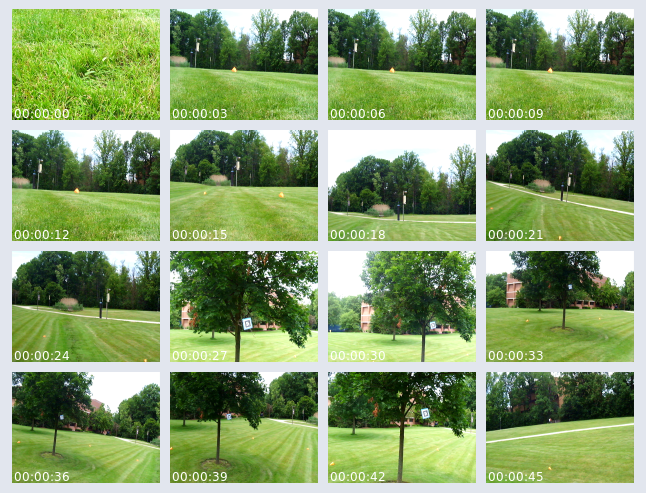
\includegraphics[scale=0.50]{./Resources/thumb_video10_l.png}
	\caption{Cenário 1 - Ambiente Externo - Árvore}
	\label{thumb_video10_l}
\end{figure}


%-----------------------------------------------------------------------------------------------------------------------------------------------------------------------------------------------
\subsubsection{Cenário 2}

O cenário da figura \ref{thumb_video12_l} foi utilizado para estudo das condições de ambiente interno, o qual também apresenta certa variação de luminosidade, porém apresenta um número maior de movimentos, permitindo uma análise de objetos estáticos à curta e média distância. Os principais obstáculos deste cenário são uma mesa, uma cadeira e duas estantes.

\begin{figure}[H]
	\centering
	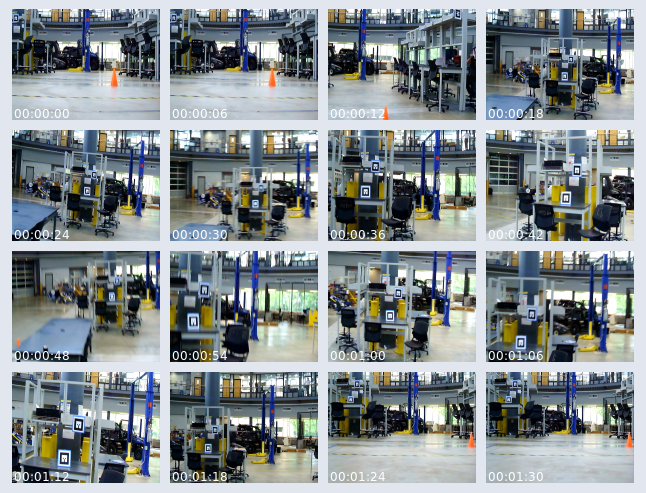
\includegraphics[scale=0.50]{./Resources/thumb_video12_l.png}
	\caption{Cenário 2 - Ambiente Interno - Mesa/Cadeira/Estantes}
	\label{thumb_video12_l}
\end{figure}


%-----------------------------------------------------------------------------------------------------------------------------------------------------------------------------------------------
\subsubsection{Cenário 3}

O cenário da figura \ref{thumb_video15} foi utilizado para estudo das condições de ambiente interno, o qual também apresenta certa variação de luminosidade, apresenta um número muito maior de movimentos e permite a análise de objetos móveis à curto e médio alcance. Os principais obstáculos deste cenário  é uma bancada e um outro quadricóptero no campo de visão do veículo pilotado.

\begin{figure}[H]
	\centering
	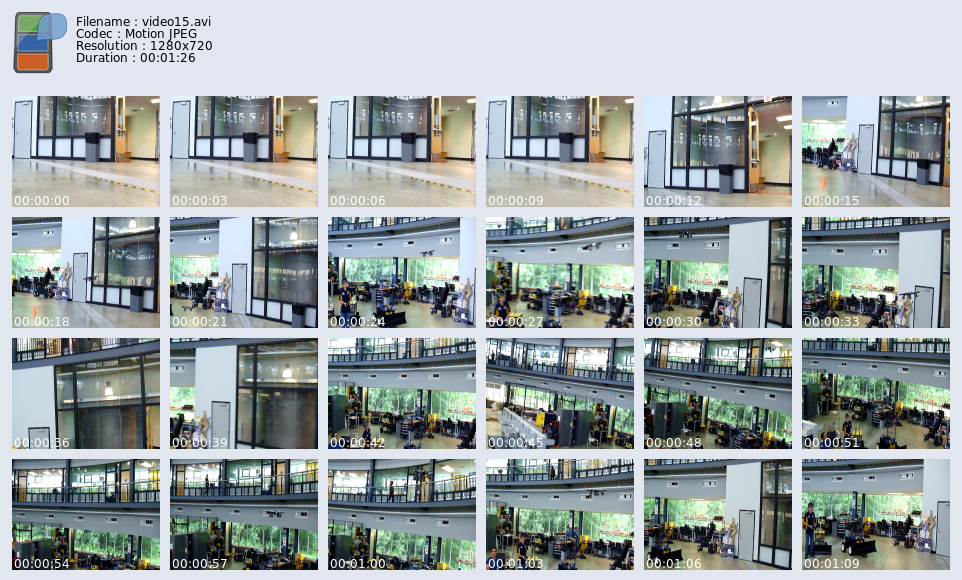
\includegraphics[scale=0.50]{./Resources/thumb_video15.png}
	\caption{Cenário 3 - Bancada/Quadricóptero}
	\label{thumb_video15}
\end{figure}


%-----------------------------------------------------------------------------------------------------------------------------------------------------------------------------------------------
\subsection{Processamento de Imagem}

Nessa seção será apresentado o processamento de imagens utilizado para a identificação de obstáculos. Como pode ser visto na figura \ref{stereo_processor_steps}, todo o processo conta com seis etapas.

\textbf{Câmeras:} O primeiro passo do processo é a captura das imagens da câmera estereoscópica. Idealmente, as imagens deve ser capturadas ao mesmo instante e as lentes não apresentarem distorções.   

\textbf{Calibração e Retificação:} Na prática, as lentes apresentam distorção. Com base nos parâmetros obtidos após a calibração das câmeras é possível retificá-las. 

\textbf{Correspondência Estéreo:} Aplica-se os métodos para encontrar as correspondências entre as duas câmeras, gerando assim o mapa de disparidades.

\textbf{Pré-filtragem:} Este passo, pode ser aplicado tanto nas imagens retificados ou no mapa de disparidades. Atualmente, aplica-se a operação morfológica de abertura e um filtro de Mediana sobre o mapa de disparidades. 

\textbf{Limiarização por Distância:} Visto que a disparidade apresenta uma relação com a distância, aplica-se uma operação de limiarização. Deste modo, apenas os obstáculos a uma certa distância são segmentados.

\textbf{Identificação de Obstáculos:} Após o passo anterior, o objeto é identificado e sua posição é rastreada. Essa informação pode ser utilizada pelo sistema de controle da aeronave para manter distância do obstáculo identificado.

\begin{figure}[H]
	\centering
	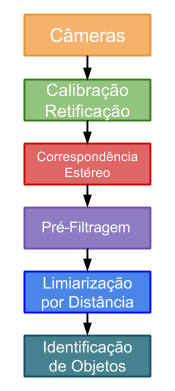
\includegraphics[scale=0.50]{./Resources/stereo_processor_steps.png}
	\caption{Etapas do Processamento de Imagens}
	\label{stereo_processor_steps}
\end{figure}


%-----------------------------------------------------------------------------------------------------------------------------------------------------------------------------------------------
\section{Correspondência Estéreo - \textit{Stereo Correspondence}}

\subsubsection{Método Estéreo - \textit{Block Matching} - BM}

\subsubsection{Método Estéreo Semi-global - \textit{Semi-global Block Matching} - SGBM}

\subsubsection{Método Estéreo Local com Aceleração de GPU - \textit{Block Matching with GPU Acceleration} - BMGPU}

%-----------------------------------------------------------------------------------------------------------------------------------------------------------------------------------------------
\subsection{Aceleração em Hardware - \textit{Hardware Acceleration}}
\subsubsection{CUDA}

\textit{Compute Unified Device Architecture} (CUDA) é uma tecnologia desenvolvida pela NVIDIA e em sua essência é uma plataforma de computação paralela de propósito geral, cujo objetivo é tirar proveito das unidades de processamento gráfico(GPU), assim, acelerando consideralmente a execução de algoritmos computacionais complexos ao comparar-se com o desempenho da CPU.

Atualmente, a maioria das placas de video da NVIDIA contam com essa tecnologia, por conta disso os pesquisadores e desenvolvidores de software estão voltando suas pesquisas para o desenvolvimento e otimização de algoritmos que possam explorar todo o poder de processamento destes dispositivos. Alguns exemplos de aplicações são identificação de placas ocultas em artérias, análise do fluxo de tráfego aéreo e visualização de moléculas

Historicamente, a implementação de algoritmos em GPU mostrou-se bastante obscura, visto que sua programação era bastante atrelada ao hardware a ser utilizado, mesmo com linguagens de programação gráfica como o OpenGL. Em 2003, um grupo de pesquisadores de Stanford, apresentaram o primeiro compilador, Brook, que facilitaria a implementação de software, visto que permitia a lidar de uma maneira mais maleável o fluxo de dados, podendo principalmente paralelizá-los. Em 2006, a NVIDIA juntamente com Ian Buck, criador do Brook, desenvolveram uma plataforma (CUDA) mais intuitiva e que permitisse a utilização de uma linguagem de alto nível e tornasse a GPU em um processador de propósito geral (GPGPU)\cite{NVIDIA}.

Neste trabalho, utilizou-se diferentes versões desta plataforma para o desenvolvimento para \textit{Desktop} e Jetson TK1. Neste contexto, essas versões não oferencem nenhuma alteração visível, visto que não foi desenvolvido nenhum tipo de rotina espeficamente para execução em GPU. Na verdade, utilizou-se as funções disponíveis na biblioteca OpenCV, as quais opcionalmente podem ser executadas pela CPU ou GPU. A tabela \ref{cudaopencv} informa as versões do pacote de ferramentas da plataforma CUDA e da biblioteca OpenCV utilizadas. 

\begin{table}[]
\centering
\caption{Versões utilizadas de CUDA e OpenCV}
\label{cudaopencv}
\begin{tabular}{cccll}
                     & \textbf{CUDA ToolKit}	     & \textbf{OpenCV} 	       &  &  \\
\textbf{Desktop}     & 7.5                           & 3.0.0                   &  &  \\
\textbf{Jetson TK1}  & 6.5                           & 2.4.12                  &  &  \\
\multicolumn{1}{l}{} & \multicolumn{1}{l}{}          & \multicolumn{1}{l}{}    &  & 
\end{tabular}
\end{table}

%-----------------------------------------------------------------------------------------------------------------------------------------------------------------------------------------------
\subsubsection{NEON}


%-----------------------------------------------------------------------------------------------------------------------------------------------------------------------------------------------
\subsection{Jetson TK1 - Configuração da Plataforma}

A execução das rotinas de visão estereoscópica com aceleração em hardware via GPU requisitam que a plataforma de desenvolvimento esteja corretamente configurada. Abaixo encontra-se o tutorial para condicioná-la para a operação desejada, isto é,basicamente, configurá-la para o correto funcionamento da CUDA e do OpenCV. 

\begin{enumerate}
  \item Baixe e instale o JetPack L4T
    \begin{enumerate}
      \item Clique \href{http://docs.nvidia.com/jetpack-l4t/index.html#developertools/mobile/jetpack/jetpack_l4t/2.1/jetpack_l4t_install.htm}{aqui} para ir ser redirecionado para a página do pacote de desenvolvimento Jetpack L4T. Caso o link esteja quebrado, vá até o página da NVIDIA e procure pelo localização correta do pacote.  

      \item Na máquina \textit{Host} rodando Ubuntu, crie um novo diretório para armazenar os pacotes de instalação utilizando as seguintes linhas de comando.
      \begin{lstlisting}[basicstyle=\tiny]
	$ ubuntu@ubuntu:~$ cd /home/<user>
	$ ubuntu@ubuntu:~/home/<user>$ mkdir flash
	$ ubuntu@ubuntu:~/home/<user>$ cd flash
	$ ubuntu@ubuntu:~/home/<user>/flash$ 
      \end{lstlisting}
      Uma ação importante que merece destaque é baixar o arquivo JetPack-\${VERSION}.run dentro do diretório criado (o caminho NÃO DEVE conter espaços).
      
      \item Dê permissão de execução para o arquivo baixado. 
      \begin{lstlisting}[basicstyle=\tiny]
	$ ubuntu@ubuntu:~/home/<user>/flash$ chmod +x JetPack-${VERSION}.run
	$ ubuntu@ubuntu:~/home/<user>/flash$ ./JetPack-${VERSION}.run
      \end{lstlisting}
      
      
    \end{enumerate}
  \item Sigua as instruções no manual de usuário do kit de desenvolvimento da Jetson TK1
    \begin{enumerate}
     \item Baixe o guia de instruções no seguinte link e clique na aba "\textit{Install Guide}". Link: \url{https://developer.nvidia.com/embedded/jetpack}
    \end{enumerate}

\end{enumerate}



% a) Download the Instruction Guide on the following link
%    link: https://developer.nvidia.com/embedded/jetpack
% b) Follow the Jetpack L4T Installer instructions
% 
% Hints: The Host Computer and the Target device(Jetson TK1) MUST be connected to the same network. This can be done by connecting:
% 1) Host PC and the target device to the same Intranet, in case the target device have a static IP address.
% 	----------------------------------------------------
% 	Editar o /etc/network/interfaces:
% 	----------------------------------------------------
% 	auto lo
% 	iface lo inet loopback
% 	auto eth0
% 	iface eth0 inet static
% 	address 10.235.0.133
% 	netmask 255.255.252.0
% 	network 10.235.3.0
% 	gateway 10.235.0.1
% 	pre-up ifconfig eth0 hw ether 00:01:02:03:05:09
% 	dns-nameservers  143.107.225.6 143.107.182.2 8.8.8.8
% 	----------------------------------------------------
% 2) Host PC and the target device to the same router. In this case, the target device must be able to find the IP address by DHCP protocol.
% 	----------------------------------------------------
% 	Editar o /etc/network/interfaces:
% 	----------------------------------------------------    
% 	auto eth0
%     	allow-hotplug eth0
%     	iface eth0 inet dhcp
% 
% ----------------------------------------------------
% 4) Installing OpenCV (including the GPU module) on Jetson TK1
% ----------------------------------------------------
% 
% First you should download & install the CUDA Toolkit by following the Installing CUDA instructions, since it is needed by OpenCV.
% And if you haven't already added the "universe" repository to your system, do it now since you will need it for some OpenCV dependencies:
% 
% \$ sudo apt-add-repository universe
% \$ sudo apt-get update
% 
% Once you have installed the CUDA Toolkit, you can begin to install OpenCV. You have several options (deciding between prebuilt library vs building the library from source, and then deciding whether to compile your code onboard the Jetson TK1 or cross-compile it from your desktop).
% Prebuilt OpenCV library versus Building the OpenCV library from source
% There are two compatible implementations of OpenCV available for Jetson TK1, but only the first option gives you the CPU optimized library, so you are highly recommended to use this first option:
% 
% Option 1) Prebuilt OpenCV4Tegra library for L4T:
% 	OpenCV4Tegra is a CPU & GPU optimized version of OpenCV, available as a prebuilt library in JetPack or as separate .deb packages (available for L4T rel-19 and L4T rel-21).
% 	eg: For OpenCV v2.4.10.1, run the following commands to manually install the prebuilt packages:
% 	Under L4T 19.x:
% 
% 	\$ sudo dpkg -i libopencv4tegra_2.4.10.1_armhf.deb
% 	\$ sudo dpkg -i libopencv4tegra-dev_2.4.10.1_armhf.deb
% 
% 	Under L4T 21.x:
% 	\$ sudo dpkg -i libopencv4tegra-repo_l4t-r21_2.4.10.1_armhf.deb
% 	\$ sudo apt-get update
% 	\$ sudo apt-get install libopencv4tegra libopencv4tegra-dev
% 
% 	Continue to the "Testing OpenCV" section lower in this page to ensure OpenCV4Tegra works on your device.
% 
% Option 2) Building the public OpenCV library from source:
% 	If you want the latest OpenCV code, or you want to customize the OpenCV library, and don't want NVIDIA's CPU & multi-core optimizations of OpenCV4Tegra, then follow the instructions below to 		compile the OpenCV library from source code. Note that you won't obtain the full performance of OpenCV4Tegra.
% 
% 	Note about SIFT/SURF in the nonfree module: OpenCV4Tegra doesn't include the opencv_nonfree package (containing SIFT & SURF feature detectors) since those algorithms are patented by other companies 		and therefore anyone using opencv_nonfree is at risk of liability.
% 	If you need something from the nonfree module, you have 2 options:
% 	Analyze the public OpenCV source code then copy/paste the parts of the nonfree module that you want (eg: SURF feature detector) from OpenCV into your own project. You will have the CPU 		optimizations of OpenCV4Tegra for most of your code and will have the GPU module and will have the non-optimized patented code that you need from the nonfree package such as SURF. So this option 		gives full performance (for everything except the nonfree code) but is tedious.
% 	Ignore OpenCV4Tegra, and instead, download & build public OpenCV (by following the instructions below for natively compiling the OpenCV library from source). You will still have the GPU module but 		not any CPU optimizations, but you won't need to spend time ripping out parts of the OpenCV non-free module code. So this option is easiest but produces slower code if you are running most of your 		code on CPU.
% 
% ----------------------------------------------------
% Referências
% ----------------------------------------------------
% Jetpack 2.0 Install on NVIDIA Jetson TK1 - https://www.youtube.com/watch?v=J-ma4aZyqfY
% Installing OpenCV (including the GPU module) on Jetson TK1 - http://elinux.org/Jetson/Installing_OpenCV

